% Results document for the time series research harness (Part 1 of the research plan).
%
% Build (from report/):   pdflatex results && pdflatex results
% Regenerate tables, figures and quoted numbers first (from the repository root):
%     uv run python scripts/make_report.py
%
% Prose is written by hand; every number comes from tables/*.tex, tables/numbers.tex
% and figures/*.pdf, which make_report.py generates from the run folders.
% What goes into this document, and what only into the run index: section
% "How this document works" (D98).

\documentclass[11pt,a4paper]{article}
\usepackage[T1]{fontenc}
\usepackage[utf8]{inputenc}
\IfFileExists{lmodern.sty}{\usepackage{lmodern}}{}  % Latin Modern fonts where installed
\usepackage[margin=2.4cm]{geometry}
\usepackage{amsmath}
\usepackage{booktabs}
\usepackage{longtable}
\usepackage{array}
\usepackage{graphicx}
\usepackage{adjustbox}  % generated tables shrink to the text width if needed
\usepackage{xcolor}
\usepackage{enumitem}
\usepackage[section]{placeins}  % floats stay in their section
\usepackage[hidelinks]{hyperref}

\graphicspath{{figures/}}
% Generated by scripts/make_report.py - do not edit by hand.
\newcommand{\BandAeCoreRpm}{0.96--0.99}
\newcommand{\BandAePeakHigh}{24.0~dB at 100 kHz}
\newcommand{\BandAePeakLow}{24.4~dB at 25.12 kHz}
\newcommand{\BandAeTopDb}{$-0.02$}
\newcommand{\BandAeTopRpm}{$-0.72$ to $-0.64$}
\newcommand{\BandAnalysed}{3,704}
\newcommand{\BandExcluded}{5}
\newcommand{\BandKappaMax}{1.651}
\newcommand{\BandKappaMin}{0.045}
\newcommand{\BandNoise}{126}
\newcommand{\BandSweeps}{3,964}
\newcommand{\BandUsLowDb}{35--49}
\newcommand{\BandUsMidDb}{0.6--2.6}
\newcommand{\BandUsMidKappa}{0.53--0.81}
\newcommand{\BandUsMidRpm}{0.62--0.85}
\newcommand{\BandZero}{129}
\newcommand{\FdbSpecLogreg}{0.943}
\newcommand{\FdbSpecSvm}{0.999}
\newcommand{\FordaFftLogTen}{0.933}
\newcommand{\FordaMinirocketFit}{0.08~s}
\newcommand{\FordaMinirocketRidge}{$0.946 \pm 0.003$}
\newcommand{\FordaPatchtstDiffLogHundred}{$-0.091$}
\newcommand{\FordaPatchtstDiffLogOne}{$-0.248$}
\newcommand{\FordaPatchtstDiffLogTen}{$-0.139$}
\newcommand{\FordaPatchtstDiffSvmHundred}{$-0.071$}
\newcommand{\FordaPatchtstDiffSvmOne}{$-0.160$}
\newcommand{\FordaPatchtstDiffSvmTen}{$-0.128$}
\newcommand{\FordaPatchtstNegLogHundred}{3}
\newcommand{\FordaPatchtstNegLogOne}{3}
\newcommand{\FordaPatchtstNegLogTen}{3}
\newcommand{\FordaPatchtstNegSvmHundred}{3}
\newcommand{\FordaPatchtstNegSvmOne}{3}
\newcommand{\FordaPatchtstNegSvmTen}{3}
\newcommand{\FordaTlossDiffLogHundred}{$-0.018$}
\newcommand{\FordaTlossDiffLogOne}{$-0.007$}
\newcommand{\FordaTlossDiffLogTen}{$-0.021$}
\newcommand{\FordaTlossDiffSvmHundred}{$-0.014$}
\newcommand{\FordaTlossDiffSvmOne}{$+0.023$}
\newcommand{\FordaTlossDiffSvmTen}{$-0.014$}
\newcommand{\FordaTlossEarlier}{0.933}
\newcommand{\FordaTlossFit}{12.4~min}
\newcommand{\FordaTlossNegLogHundred}{3}
\newcommand{\FordaTlossNegLogOne}{2}
\newcommand{\FordaTlossNegLogTen}{3}
\newcommand{\FordaTlossNegSvmHundred}{3}
\newcommand{\FordaTlossNegSvmOne}{1}
\newcommand{\FordaTlossNegSvmTen}{3}
\newcommand{\FordaTsjepaDiffLogHundred}{$+0.002$}
\newcommand{\FordaTsjepaDiffLogOne}{$+0.012$}
\newcommand{\FordaTsjepaDiffLogTen}{$-0.001$}
\newcommand{\FordaTsjepaDiffSvmHundred}{$-0.001$}
\newcommand{\FordaTsjepaDiffSvmOne}{$+0.024$}
\newcommand{\FordaTsjepaDiffSvmTen}{$+0.010$}
\newcommand{\FordaTsjepaNegLogHundred}{1}
\newcommand{\FordaTsjepaNegLogOne}{1}
\newcommand{\FordaTsjepaNegLogTen}{1}
\newcommand{\FordaTsjepaNegSvmHundred}{2}
\newcommand{\FordaTsjepaNegSvmOne}{1}
\newcommand{\FordaTsjepaNegSvmTen}{0}
\newcommand{\FordaTsvecDiffLogHundred}{$-0.017$}
\newcommand{\FordaTsvecDiffLogOne}{$+0.002$}
\newcommand{\FordaTsvecDiffLogTen}{$-0.029$}
\newcommand{\FordaTsvecDiffSvmHundred}{$-0.010$}
\newcommand{\FordaTsvecDiffSvmOne}{$+0.028$}
\newcommand{\FordaTsvecDiffSvmTen}{$-0.011$}
\newcommand{\FordaTsvecEarlier}{0.932}
\newcommand{\FordaTsvecFit}{24.20~s}
\newcommand{\FordaTsvecFitFirst}{30~s}
\newcommand{\FordaTsvecFitRest}{23--24~s}
\newcommand{\FordaTsvecLogTen}{0.904}
\newcommand{\FordaTsvecNegLogHundred}{3}
\newcommand{\FordaTsvecNegLogOne}{1}
\newcommand{\FordaTsvecNegLogTen}{3}
\newcommand{\FordaTsvecNegSvmHundred}{3}
\newcommand{\FordaTsvecNegSvmOne}{0}
\newcommand{\FordaTsvecNegSvmTen}{3}
\newcommand{\MinirocketAcc}{$0.946 \pm 0.003$}
\newcommand{\MinirocketVerdict}{pass}
\newcommand{\TfcFullDiverged}{4}
\newcommand{\TfcFullFirstIdentical}{identical}
\newcommand{\TfcFullIdentical}{identical}
\newcommand{\TfcFullResultsWritten}{no}
\newcommand{\TfcFullSeeds}{5}
\newcommand{\TfcOursAcc}{$0.706 \pm 0.112$}
\newcommand{\TfcOursAccMax}{0.803}
\newcommand{\TfcOursAccMin}{0.519}
\newcommand{\TfcOursFone}{$0.757 \pm 0.089$}
\newcommand{\TfcOursNval}{21}
\newcommand{\TfcOursVerdict}{pass}
\newcommand{\TfcProbePreLogreg}{$0.961 \pm 0.012$}
\newcommand{\TfcProbePreSvm}{$0.951 \pm 0.021$}
\newcommand{\TfcProbeRandLogreg}{$0.738 \pm 0.091$}
\newcommand{\TfcProbeRandSvm}{$0.973 \pm 0.020$}
\newcommand{\TfcSubsetAcc}{$0.382 \pm 0.164$}
\newcommand{\TfcSubsetFone}{$0.178 \pm 0.069$}
\newcommand{\TfcSubsetVerdict}{fail}
\newcommand{\TlossAcc}{$0.932 \pm 0.007$}
\newcommand{\TlossVerdict}{pass}
\newcommand{\TsjepaAcc}{$0.941 \pm 0.005$}
\newcommand{\TsjepaVerdict}{fail}
\newcommand{\TsvecAcc}{$0.936 \pm 0.003$}
\newcommand{\TsvecVerdict}{pass}
  % generated numbers quoted in the prose

\setlist{nosep, leftmargin=*}
\setlength{\parskip}{4pt}
\setlength{\parindent}{0pt}
\setlength{\LTcapwidth}{\linewidth}
\setlength{\emergencystretch}{3em}  % fewer overfull lines with long file names

% --- Entry layout -----------------------------------------------------------
\definecolor{muted}{HTML}{8a8984}
\definecolor{openpt}{HTML}{b4451f}
% \entry{label}{title}{date}{decisions}{run folders}
\newcommand{\entry}[5]{%
  \subsection{#2}\label{#1}
  \begin{tabular}{@{}>{\footnotesize\color{muted}}l>{\footnotesize}p{0.8\linewidth}@{}}
    Date & #3 \\ Decisions & #4 \\ Runs & #5
  \end{tabular}\par}
\newcommand{\question}{\paragraph{Question.}}
\newcommand{\test}{\paragraph{Test.}}
\newcommand{\result}{\paragraph{Result.}}
\newcommand{\finding}{\paragraph{Finding.}}
\newcommand{\consequence}{\paragraph{Consequence.}}
\newcommand{\openpoint}[1]{\par\textcolor{openpt}{\textbf{Open:}} #1\par}
\newcommand{\run}[1]{\texttt{\detokenize{#1}}}
\newcommand{\sref}[1]{\S\ref{#1}}

\title{Results\\[2pt]\large Time series research harness --- Part 1: evaluation harness and baselines}
\author{}
\date{Generated \today}

\begin{document}
\maketitle
\tableofcontents

% =============================================================================
\section{How this document works}

This document reports the current results of the project, organised by topic: for each
result, the question it answers, how it was tested, what came out, and what was concluded
or decided from it. Design decisions themselves live in \texttt{DECISIONS.md} and
\texttt{decisions/} (cited as D$n$); open questions for supervision in
\texttt{QUESTIONS.md} (Q$n$). How the document is kept is decided in D98.

\textbf{Current results only.} When a run is replaced (for example a rerun of the same
configuration), its result leaves the text. Where a later result builds on it, it is kept
as a sentence (``an earlier run gave~\ldots''), not as an entry of its own.

\textbf{Every run stays findable.} All tables, figures and numbers quoted in the text are
generated by \path{scripts/make_report.py} from the run folders (\texttt{runs/}, not
committed); each entry names its run folders. The run index
(Appendix~\ref{app:runs}) lists every folder in \texttt{runs/}, including superseded,
empty and not-yet-written-up runs, with what it was for, its status, commit and device.

\textbf{Conventions.} Unless stated otherwise: mean $\pm$ standard deviation over seeds
(sample SD, $n-1$); the test set is scored once; accuracies are fractions, not
percentages.

\textbf{Reproduction criterion} (D26 item 6, also used in D38). Implemented in
\texttt{scripts/evaluate.py} and \texttt{scripts/tfc\_official.py} as
\[
  |\text{published} - \text{mean}| \;\le\; \max(2\,\mathrm{SD},\ 0.01).
\]

% Generated by scripts/make_report.py - do not edit by hand.
\begin{table}[htbp]
\centering
\small
\caption{Reproduction checks: published accuracy against our mean over seeds, with the method's own probe and all labels. Criterion as implemented in \texttt{scripts/evaluate.py} and \texttt{scripts/tfc\_official.py} (D26, D38): pass if $|\Delta| \le \max(2\,\mathrm{SD}, 0.01)$.}
\label{tab:repro}
\begin{adjustbox}{max width=\linewidth}
\begin{tabular}{lllccccc}
\toprule
Section & Method & Data & Published & Ours (mean $\pm$ SD) & $|\Delta|$ & Allowed & Criterion \\
\midrule
\ref{forda-repro} & TS2Vec & FordA & 0.9360 & $0.936 \pm 0.003$ ($n=3$) & 0.000 & 0.010 & pass \\
\ref{forda-repro} & T-Loss & FordA & 0.9280 & $0.932 \pm 0.007$ ($n=3$) & 0.004 & 0.015 & pass \\
\ref{forda-repro} & MiniRocket & FordA & 0.9500 & $0.946 \pm 0.003$ ($n=3$) & 0.004 & 0.010 & pass \\
\ref{forda-repro} & TS-JEPA, official masking & FordA & 0.9150 & $0.941 \pm 0.005$ ($n=3$) & 0.026 & 0.010 & fail \\
\ref{tfc-full} & TF-C, official, full data & FD & 0.8934 & no test result & -- & -- & -- \\
\ref{tfc-ours} & TF-C, ours & FD & 0.8934 & $0.706 \pm 0.112$ ($n=5$) & 0.187 & 0.224 & pass \\
\ref{tfc-subset} & TF-C, official, subset & FD & 0.8934 & $0.382 \pm 0.164$ ($n=5$) & 0.511 & 0.327 & fail \\
\bottomrule
\end{tabular}
\end{adjustbox}
\end{table}


% =============================================================================
\section{Data layer}

\entry{data-conversion}{Conversions reproduce the source values}{2026-10-07 -- 2026-10-08}
  {D3, D5, D20--D25, D27, D30, D39, D44}{none (unit tests; see below)}

\question
Does the conversion to the canonical format (D3, D5) return exactly the values in the
source files?

\test
\begin{itemize}
  \item Herning (\texttt{tests/test\_herning.py}): the first 20 sweeps of
        \run{scope_20260901_112732.h5} are converted into a temporary folder; every sample
        of both channels (AE, UL) is compared with the source (absolute tolerance
        $10^{-9}$, far below one code step), and a slice must equal the corresponding part
        of the full signal. The test also checks four tables, one telemetry row per
        capture, two channels and time order.
  \item FordA: converted values compared with the archive's text files.
  \item FD-A: checked for non-finite values before the TF-C divergence was investigated (D44).
\end{itemize}

\result
Herning conversion exact on the 20 sweeps tested; FordA exact against the files; FD-A
contains no non-finite values. These outcomes are recorded in \texttt{HANDOFF.md} and
D44; no test log is stored.

\finding
The data layer can be trusted for the runs below. The full Herning run has not yet been
converted; the band check (\sref{band-check}) reads the source file directly.

\openpoint{Test outcomes are not stored anywhere but in notes. Should test runs write a
log (e.g.\ into \texttt{runs/}) so that this entry can cite one?}

% =============================================================================
\section{Public benchmark: FordA}

FordA (UCR archive, used as distributed: D27, D30) is the first benchmark: frozen
representations, the harness probes (D26), three seeds, label budgets 1\,\%, 10\,\% and
100\,\% (D29, D40). It validates the harness against published numbers and sets the bar
the SSL methods have to clear against simple baselines (D75). All runs in this section were
made on the work computer on 2026-10-20, one after another, with timing (D79). The working
tree had uncommitted changes when they started (the baseline code, committed afterwards;
Table~\ref{tab:runs}).

\entry{forda-repro}{TS2Vec, T-Loss and MiniRocket reproduce their published accuracies}{2026-10-20}
  {D26, D28, D32, D76, D79, D81}{\run{20261020_144711_ts2vec_forda}, \run{20261020_144932_tloss_forda},
  \run{20261020_152809_minirocket_forda}}

\question
Do the methods, wrapped from their official code with the official settings, reproduce the
published FordA accuracies with their own probes?

\test
TS2Vec with the official defaults (D28; 600 iterations, 320-dimensional representation
max-pooled over time); T-Loss with its official settings (D32; 2,000 steps, $K = 10$);
MiniRocket with the official code and settings (D76, D81; 9,996 features). Each is probed with
its own protocol and all training labels: the RBF-SVM protocol of TS2Vec (also T-Loss's own),
and MiniRocket's ridge classifier (D81). Published targets: TS2Vec 0.936 (batch size 8),
T-Loss 0.928, MiniRocket 0.950 (official results file, resample 0, taken to be the original
split, D81). Three seeds; TS2Vec and T-Loss on the GPU, MiniRocket on the CPU.

\result
TS2Vec \TsvecAcc{} (\TsvecVerdict), T-Loss \TlossAcc{} (\TlossVerdict), MiniRocket
\MinirocketAcc{} (\MinirocketVerdict); Table~\ref{tab:repro}. Earlier runs of the same
TS2Vec and T-Loss configurations (2026-10-08, without timing; run index) gave
\FordaTsvecEarlier{} and \FordaTlossEarlier: a rerun moves the mean by a few thousandths.

\finding
All three reproduce, so the wrapped methods and the evaluation pipeline can be trusted on
FordA.

\entry{forda-baselines}{SSL methods against training-free baselines: the baselines win except at 1\,\% labels}{2026-10-20}
  {D75--D80, D83, D85, D89, D90}{\run{20261020_143928_raw_forda}, \run{20261020_144122_fft_forda},
  \run{20261020_144235_catch22_forda}, \run{20261020_152809_minirocket_forda},
  \run{20261020_144711_ts2vec_forda}, \run{20261020_144932_tloss_forda}}

\question
Do TS2Vec and T-Loss beat simple baselines on FordA, in accuracy, with few labels, and in
speed (D75)?

\test
Baselines (D75): the floor (most frequent class, D83); the raw samples, probed with the SVM
only (D89); the one-sided linear $|$FFT$|$ spectrum (D76); catch24, i.e.\ catch22 plus mean
and SD, from pycatch22 1.0.2 (D85, D90); and MiniRocket (D76, D81). Every baseline goes
through the same probes, label budgets and seeds (0, 1, 2) as the SSL methods, so at each
budget all methods are probed on the same labelled series (D78). Comparison: per probe and
budget, each SSL method's paired difference to the best baseline (D80). Timing: wall-clock
per stage (D79), median over seeds.

\result
Accuracies in Table~\ref{tab:forda-accuracy} and Figure~\ref{fig:forda}; paired differences
in Table~\ref{tab:forda-paired}; times in Table~\ref{tab:forda-timing}.
\begin{itemize}
  \item 10\,\% and 100\,\% labels: the best baseline is ahead of both SSL methods with both
        probes, in every seed. With the logistic probe at 10\,\%, $|$FFT$|$ reaches
        \FordaFftLogTen{} against \FordaTsvecLogTen{} for TS2Vec (paired difference
        \FordaTsvecDiffLogTen; T-Loss \FordaTlossDiffLogTen).
  \item 1\,\% labels: with the SVM probe, TS2Vec and T-Loss are ahead of $|$FFT$|$ by
        \FordaTsvecDiffSvmOne{} and \FordaTlossDiffSvmOne, largely from seed~0. With the
        logistic probe they tie with MiniRocket (\FordaTsvecDiffLogOne{} and
        \FordaTlossDiffLogOne).
  \item Speed: per seed, MiniRocket fits in \FordaMinirocketFit{} on the CPU, TS2Vec trains in
        \FordaTsvecFit{} and T-Loss in \FordaTlossFit{} on the GPU. $|$FFT$|$ and catch24 fit
        nothing. The slowest step for MiniRocket is the SVM probe on its 9,996 features.
  \item catch24 is the weakest baseline after the raw samples, and its spread at 1\,\% labels
        is large.
\end{itemize}

\finding
On FordA, pretraining pays off only with 1\,\% labels, and there only with the SVM probe and
not in every seed. Otherwise the training-free baselines are as good or better, at a small
fraction of the cost. FordA's classes are well separated by the spectrum, so this need not
carry over to the rig data; it sets the bar: an SSL method has to beat $|$FFT$|$ and
MiniRocket, not only the floor.

\openpoint{TS-JEPA and PatchTST have been run on FordA but are not yet in this comparison
(run index). The untrained-encoder control (D75 f) has not been run. On the GPU the first
seed includes start-up time (TS2Vec: \FordaTsvecFitFirst{} against \FordaTsvecFitRest{} for the
others); the table reports the median.}

% Generated by scripts/make_report.py - do not edit by hand.
\begin{table}[htbp]
\centering
\small
\caption{FordA test accuracy, frozen representations: mean $\pm$ SD over 3 seeds; the same labelled series for every method at each budget (D78). Bold: best mean per column. Raw samples are not probed with logistic regression (D89). The floor ignores the features, so it is the same under both probes (D83).}
\label{tab:forda-accuracy}
\begin{adjustbox}{max width=\linewidth}
\begin{tabular}{lcccccc}
\toprule
 & \multicolumn{3}{c}{Logistic regression} & \multicolumn{3}{c}{SVM (TS2Vec protocol)} \\
Method & 1\,\% & 10\,\% & 100\,\% & 1\,\% & 10\,\% & 100\,\% \\
\midrule
TS2Vec & $\mathbf{0.862} \pm 0.022$ & $0.904 \pm 0.011$ & $0.929 \pm 0.004$ & $\mathbf{0.876} \pm 0.025$ & $0.914 \pm 0.006$ & $0.936 \pm 0.003$ \\
T-Loss & $0.853 \pm 0.018$ & $0.912 \pm 0.006$ & $0.928 \pm 0.004$ & $0.871 \pm 0.018$ & $0.911 \pm 0.007$ & $0.932 \pm 0.007$ \\
\midrule
Raw samples & not run & not run & not run & $0.558 \pm 0.035$ & $0.669 \pm 0.008$ & $0.828 \pm 0.000$ \\
$|$FFT$|$ & $0.829 \pm 0.011$ & $\mathbf{0.933} \pm 0.004$ & $0.939 \pm 0.000$ & $0.848 \pm 0.018$ & $\mathbf{0.925} \pm 0.005$ & $0.945 \pm 0.000$ \\
catch24 & $0.664 \pm 0.129$ & $0.830 \pm 0.010$ & $0.843 \pm 0.000$ & $0.602 \pm 0.104$ & $0.838 \pm 0.004$ & $0.880 \pm 0.000$ \\
MiniRocket & $0.860 \pm 0.032$ & $0.923 \pm 0.007$ & $\mathbf{0.945} \pm 0.004$ & $0.795 \pm 0.041$ & $0.917 \pm 0.003$ & $\mathbf{0.946} \pm 0.001$ \\
\midrule
Floor (most frequent class) & $0.516$ & $0.516$ & $0.516$ & $0.516$ & $0.516$ & $0.516$ \\
\bottomrule
\end{tabular}
\end{adjustbox}
\end{table}

% Generated by scripts/make_report.py - do not edit by hand.
\begin{table}[htbp]
\centering
\small
\caption{FordA: paired difference in test accuracy, SSL method minus the best baseline at that probe and label budget (positive: the SSL method is better). Per seed, the two use the same labelled series (D78). The best baseline is chosen by its mean test accuracy, which favours the baselines (D80). Seeds in the order 0, 1, 2.}
\label{tab:forda-paired}
\begin{adjustbox}{max width=\linewidth}
\begin{tabular}{lllcccc}
\toprule
Probe & Labels & Best baseline (mean) & TS2Vec: mean (per seed) & T-Loss: mean (per seed) & TS-JEPA (masking fixed): mean (per seed) & PatchTST: mean (per seed) \\
\midrule
Logistic regression & 1\,\% & MiniRocket ($0.860$) & $+0.002$ \,$(-0.013, +0.011, +0.009)$ & $-0.007$ \,$(-0.021, -0.022, +0.022)$ & $+0.012$ \,$(-0.001, +0.003, +0.033)$ & $-0.248$ \,$(-0.259, -0.292, -0.192)$ \\
 & 10\,\% & $|$FFT$|$ ($0.933$) & $-0.029$ \,$(-0.035, -0.036, -0.016)$ & $-0.021$ \,$(-0.023, -0.024, -0.015)$ & $-0.001$ \,$(-0.011, +0.004, +0.005)$ & $-0.139$ \,$(-0.080, -0.152, -0.185)$ \\
 & 100\,\% & MiniRocket ($0.945$) & $-0.017$ \,$(-0.018, -0.019, -0.014)$ & $-0.018$ \,$(-0.010, -0.027, -0.017)$ & $+0.002$ \,$(+0.007, -0.011, +0.011)$ & $-0.091$ \,$(-0.040, -0.100, -0.133)$ \\
\midrule
SVM (TS2Vec protocol) & 1\,\% & $|$FFT$|$ ($0.848$) & $+0.028$ \,$(+0.067, +0.002, +0.014)$ & $+0.023$ \,$(+0.055, -0.014, +0.029)$ & $+0.024$ \,$(+0.060, -0.002, +0.016)$ & $-0.160$ \,$(-0.146, -0.203, -0.130)$ \\
 & 10\,\% & $|$FFT$|$ ($0.925$) & $-0.011$ \,$(-0.003, -0.019, -0.011)$ & $-0.014$ \,$(-0.010, -0.020, -0.011)$ & $+0.010$ \,$(+0.015, +0.006, +0.010)$ & $-0.128$ \,$(-0.077, -0.135, -0.171)$ \\
 & 100\,\% & MiniRocket ($0.946$) & $-0.010$ \,$(-0.009, -0.013, -0.009)$ & $-0.014$ \,$(-0.013, -0.021, -0.008)$ & $-0.001$ \,$(-0.002, -0.004, +0.003)$ & $-0.071$ \,$(-0.039, -0.080, -0.096)$ \\
\bottomrule
\end{tabular}
\end{adjustbox}
\end{table}

% Generated by scripts/make_report.py - do not edit by hand.
\begin{table}[htbp]
\centering
\small
\caption{FordA: wall-clock time per stage (D79), median over 3 seeds. Encoding: training and test series (4,921) per second. Probe fit includes the probe's cross-validation. Hardware: NVIDIA RTX 4500 Ada Generation GPU, 36-thread CPU. MiniRocket's code compiles once on import (0.54~s, not included, D81). TS-JEPA and PatchTST were run before timing existed (D102, D103).}
\label{tab:forda-timing}
\begin{adjustbox}{max width=\linewidth}
\begin{tabular}{llrrrr}
\toprule
 &  & Fit / pretraining (s) & Encoding & \multicolumn{2}{c}{Probe fit, 100\,\% labels (s)} \\
Method & Device & median (range) & series/s & Logistic & SVM \\
\midrule
TS2Vec & GPU & 24.20 (22.58--29.56) & 2,577 & 2.8 & 9.1 \\
T-Loss & GPU & 742.81 (738.37--756.01) & 829 & 2.9 & 9.9 \\
TS-JEPA (masking fixed) & -- & not timed & -- & -- & -- \\
PatchTST & -- & not timed & -- & -- & -- \\
Raw samples & CPU & none & 639,095,705 & -- & 30.4 \\
$|$FFT$|$ & CPU & none & 294,389 & 9.5 & 7.3 \\
catch24 & CPU & none & 1,098 & 0.7 & 73.3 \\
MiniRocket & CPU & 0.08 (0.07--0.10) & 28,549 & 33.5 & 540.7 \\
\bottomrule
\end{tabular}
\end{adjustbox}
\end{table}


\begin{figure}[htbp]
\centering
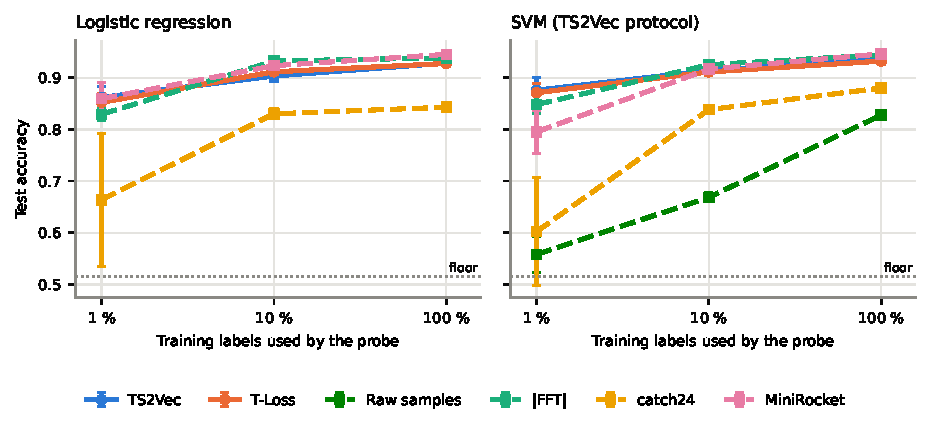
\includegraphics[width=\linewidth]{forda_label_efficiency}
\caption{FordA test accuracy against the share of training labels given to the probe, one
panel per probe. Solid lines with circles: SSL methods; dashed lines with squares: baselines;
dotted: the floor. Error bars: SD over 3 seeds. Raw samples appear only under the SVM probe
(D89). The numbers are in Table~\ref{tab:forda-accuracy}.}
\label{fig:forda}
\end{figure}

% =============================================================================
\section{\texorpdfstring{TF-C on FD-A $\rightarrow$ FD-B}{TF-C on FD-A to FD-B}}

TF-C is studied in steps (D35): (1) reproduce the published result with the official code;
(2) the official TF-C on the full, raw Paderborn data; (3) our own corrected TF-C;
(4) possibly a comparison on FordA. FD-A and FD-B are used as distributed by the TF-C
authors (D39): pretraining on FD-A (train), fine-tuning on the 60 FD-B training windows,
epoch selection on the \TfcOursNval{} FD-B validation windows, testing on FD-B test. Target:
$0.8934 \pm 0.0379$ accuracy, 5 runs (TF-C paper, Table 5; D38). The official reference is
the 2023 code (D36), run with two protocols: \emph{official} (epoch with the best
\emph{test} accuracy, as the official code) and \emph{clean} (epoch with the best
validation macro-F1, D37, D43).

\entry{tfc-full}{Official TF-C diverges on the full FD-A data}{2026-10-08}
  {D36, D37, D38, D44}{\run{20261008_134951_tfc_official_fd}, \run{20261008_143021_tfc_official_fd},
  \run{20261008_155516_tfc_official_fd}}

\question
Does the official TF-C code, run on all FD-A windows (debugging subset off, D37),
reproduce the published FD-A $\to$ FD-B accuracy?

\test
Official 2023 code through our adapter, settings checked against the official
\path{FD_A_Configs.py} (40 epochs, batch 64, learning rate $3\cdot10^{-4}$, weight decay
$3\cdot10^{-4}$ as hard-coded). Five seeds. Three attempts: the first (seed 0 only) and second
with commit \texttt{87e9222}; the third with commit \texttt{c11957a}, which records a
non-finite pretraining loss as divergence and skips fine-tuning for that seed (D44).

\result
In \TfcFullDiverged{} of \TfcFullSeeds{} seeds the pretraining loss became non-finite
(Table~\ref{tab:tfc-official-full}, Figure~\ref{fig:tfc-loss}); in the first attempt
fine-tuning then crashed. The pretraining losses of the second and third attempt are
\TfcFullIdentical{} for every seed, and the first attempt's finite losses (seed 0) are
\TfcFullFirstIdentical{} to them, so the divergence is deterministic given the seed. Seed 4
completed pretraining, but no attempt wrote fine-tuning output for it, and the third
attempt wrote no \texttt{results.csv} (results file written: \TfcFullResultsWritten).

\finding
On the full data, the official code does not produce a single test result. A likely
cause, not verified (D44): gradients are reset only once per epoch, so each step on the
full data uses many accumulated batches.

\consequence
D44: divergence is now recorded per seed as a result, and the official run was repeated
with the debugging subset (\sref{tfc-subset}).

\openpoint{Why seed 4, whose pretraining finished, has no fine-tuning output, is not
recorded in the run folder.}

% Generated by scripts/make_report.py - do not edit by hand.
\begin{table}[htbp]
\centering
\small
\caption{Official TF-C, full FD-A pretraining data (R5, third attempt). Pretraining loss per epoch is empty in \texttt{pretrain\_loss.csv} once it is no longer finite.}
\label{tab:tfc-official-full}
\begin{adjustbox}{max width=\linewidth}
\begin{tabular}{rccccc}
\toprule
Seed & Epochs run & Finite & First non-finite & Last finite loss & Fine-tuning output \\
\midrule
0 & 5 & 4 & 5 & 8.290 & no \\
1 & 22 & 21 & 22 & 8.186 & no \\
2 & 17 & 16 & 17 & 8.190 & no \\
3 & 5 & 4 & 5 & 8.340 & no \\
4 & 40 & 40 & -- & 8.185 & no \\
\bottomrule
\end{tabular}
\end{adjustbox}
\par\vspace{2pt}\parbox{0.95\linewidth}{\footnotesize Second and third attempt: pretraining losses identical for every seed.}
\end{table}


\entry{tfc-ours}{Our TF-C falls well below the published accuracy}{2026-10-08}
  {D41, D42 (D38, D39)}{\run{20261008_142751_tfc_fd}}

\question
Does our TF-C (paper's CNN and loss, corrected frequency augmentation, selection by
validation macro-F1; D41, D42) reach the published FD-A $\to$ FD-B accuracy?

\test
Settings in D41/D42 and the run's \texttt{config.yaml}. Five seeds. Component checks in
\texttt{tests/test\_tfc.py} (NT-Xent and $L_C$ equal the official functions; frequency
augmentation symmetric and the spectrum of a real signal; permutation reaches $M$
segments); their outcome is not stored with the run.

\result
Test accuracy \TfcOursAcc{}, macro-F1 \TfcOursFone{}; single seeds range from \TfcOursAccMin{} to
\TfcOursAccMax{} (Table~\ref{tab:tfc-ours}). The validation macro-F1 moves in large steps
between epochs (Figure~\ref{fig:tfc-val}); one validation window is $1/\TfcOursNval$ of the
validation set.

\finding
The mean is far below the published $0.8934$, with a large spread over seeds. Formally,
the criterion of D26 gives ``\TfcOursVerdict'', because twice the SD exceeds the gap
(Table~\ref{tab:repro}).

\consequence
D45 and D46: diagnostics to tell ``pretraining learned little'' from ``fine-tuning or
selection failed'' (\sref{tfc-probe}) and to check whether FD-B can separate methods (\sref{fdb-spectrum}).

\openpoint{The criterion passes a mean far below the target because the spread is large.
Is our TF-C result a reproduction? Should the criterion get a condition on the spread (D26 item 6
speaks of the 1-pp clause only ``if the spread is very small'', while the code applies it
always)?}

% Generated by scripts/make_report.py - do not edit by hand.
\begin{table}[htbp]
\centering
\small
\caption{Our TF-C (D41, D42), FD-A $\rightarrow$ FD-B test set. Epoch: fine-tuning epoch with the best validation macro-F1; the test set is scored once, for that epoch. Precision, recall and F1 are macro averages.}
\label{tab:tfc-ours}
\begin{adjustbox}{max width=\linewidth}
\begin{tabular}{rrcccccc}
\toprule
Seed & Epoch & Acc. & Prec. & Recall & F1 & AUROC & AUPRC \\
\midrule
0 & 26 & 0.803 & 0.857 & 0.839 & 0.847 & 0.765 & 0.738 \\
1 & 40 & 0.769 & 0.844 & 0.831 & 0.808 & 0.831 & 0.812 \\
2 & 33 & 0.519 & 0.638 & 0.648 & 0.614 & 0.732 & 0.712 \\
3 & 18 & 0.690 & 0.764 & 0.769 & 0.745 & 0.847 & 0.821 \\
4 & 30 & 0.750 & 0.752 & 0.817 & 0.769 & 0.786 & 0.758 \\
\midrule
Mean $\pm$ SD &  & $0.706 \pm 0.112$ & $0.771 \pm 0.088$ & $0.781 \pm 0.079$ & $0.757 \pm 0.089$ & $0.792 \pm 0.047$ & $0.768 \pm 0.047$ \\
\bottomrule
\end{tabular}
\end{adjustbox}
\end{table}


\begin{figure}[htbp]
\centering
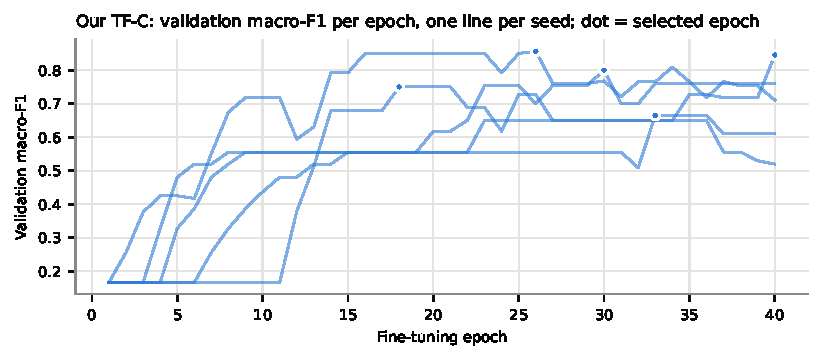
\includegraphics[width=\linewidth]{tfc_ours_validation}
\caption{Our TF-C: validation macro-F1 after every fine-tuning epoch, one line per
seed; dot: the selected epoch (first maximum).}
\label{fig:tfc-val}
\end{figure}

\entry{tfc-probe}{Frozen probes on our TF-C encoders: pretraining is not where the shortfall is}{2026-10-08}
  {D45}{\run{20261008_151014_probe_tfc_fd}}

\question
Did our TF-C pretraining (\sref{tfc-ours}) learn a representation that separates the FD-B classes, so
that the low fine-tuned accuracy comes from fine-tuning or epoch selection? Or did
pretraining learn little?

\test
The five pretrained encoders of our TF-C run are frozen; their representation $[z_T; z_F]$ is probed
with both harness probes trained on all 60 FD-B training labels and scored once on FD-B
test (D45). Reference: untrained encoders of the same architecture, initialised with the
same seeds, probed the same way. 100\,\% labels only (exception to D40: 1\,\% of 60 is
less than one window).

\result
Pretrained encoder: SVM \TfcProbePreSvm, logistic regression \TfcProbePreLogreg.
Untrained encoder: SVM \TfcProbeRandSvm, logistic regression \TfcProbeRandLogreg{}
(Table~\ref{tab:fdb}, Figure~\ref{fig:fdb}).

\finding
Probes on the frozen pretrained encoders score far above the fine-tuned TF-C (\sref{tfc-ours}), which
points to fine-tuning or epoch selection rather than pretraining. But pretraining does
not beat an untrained encoder with the SVM probe; it helps only the linear probe.

\entry{fdb-spectrum}{Plain spectra separate FD-B almost perfectly}{2026-10-08}
  {D46}{\run{20261008_162447_probe_spectrum_fd}}

\question
Can FD-B separate methods at all, given that an untrained encoder with an SVM probe
already reaches high accuracy (\sref{tfc-probe})?

\test
Both harness probes trained directly on the full FFT magnitude spectrum of each FD-B
training window (the input of TF-C's frequency branch), no encoder; 60 labels; scored once
on FD-B test. Deterministic, so one value per probe. Run in Claude's cloud workspace on
the work computer's FD-B data, copied unchanged (\texttt{NOTE.txt} in the run folder).

\result
SVM \FdbSpecSvm, logistic regression \FdbSpecLogreg{} (Table~\ref{tab:fdb}).

\finding
With 60 labels, an SVM on the plain spectrum classifies FD-B test almost without error,
above the published TF-C result. Under this protocol FD-B cannot show that a pretrained
method adds anything (the condition stated in D46's rationale is met).

\openpoint{What follows for the TF-C study (D35) from the FD-B diagnostics (\sref{tfc-probe}--\sref{tfc-subset}) has not been decided.}

\entry{tfc-subset}{Official TF-C with its debugging subset collapses to one class}{2026-10-08}
  {D37, D44 (D43)}{\run{20261008_171159_tfc_official_fd_subset}}

\question
Is the debugging subset what makes the official code trainable, and does it then
reproduce the published accuracy (D37: first check if the reproduction fails; D44)?

\test
As in \sref{tfc-full}, with the official debugging subset switched on (as shipped: 640 FD-A windows for
pretraining). Five seeds; both protocols.

\result
No seed diverged (Figure~\ref{fig:tfc-loss}). Test accuracy \TfcSubsetAcc{}, macro-F1
\TfcSubsetFone{} (official protocol; criterion: \TfcSubsetVerdict). In every seed and every
fine-tuning epoch, macro recall on test and validation is exactly $1/3$
(Table~\ref{tab:tfc-official-subset}), which is what predicting one class for every
window gives. All epochs therefore tie and both protocols select epoch 1; official and
clean numbers are identical.

\finding
With the subset the official code trains without diverging, but the fine-tuned model
predicts a single class. Neither configuration of the official code reproduces the paper.

% Generated by scripts/make_report.py - do not edit by hand.
\begin{table}[htbp]
\centering
\small
\caption{Official TF-C with the debugging subset. Official protocol: epoch with the best test accuracy; clean protocol: epoch with the best validation macro-F1 (D43). Last column: macro recall on test and validation is exactly $1/3$ at every one of the 40 fine-tuning epochs.}
\label{tab:tfc-official-subset}
\begin{adjustbox}{max width=\linewidth}
\begin{tabular}{rccccccc}
\toprule
Seed & \multicolumn{3}{c}{Official protocol} & \multicolumn{3}{c}{Clean protocol} & Recall $=1/3$ \\
\midrule
 & Epoch & Acc. & F1 & Epoch & Acc. & F1 & all epochs \\
\midrule
0 & 1 & 0.455 & 0.209 & 1 & 0.455 & 0.209 & yes \\
1 & 1 & 0.089 & 0.055 & 1 & 0.089 & 0.055 & yes \\
2 & 1 & 0.455 & 0.209 & 1 & 0.455 & 0.209 & yes \\
3 & 1 & 0.455 & 0.209 & 1 & 0.455 & 0.209 & yes \\
4 & 1 & 0.455 & 0.209 & 1 & 0.455 & 0.209 & yes \\
\bottomrule
\end{tabular}
\end{adjustbox}
\end{table}


\subsection*{FD-B results side by side}

% Generated by scripts/make_report.py - do not edit by hand.
\begin{table}[htbp]
\centering
\small
\caption{FD-B test set: TF-C results and the diagnostics. Probes use all 60 FD-B training labels (D45, D46). The $|$FFT$|$ probes are deterministic (one value).}
\label{tab:fdb}
\begin{adjustbox}{max width=\linewidth}
\begin{tabular}{llccr}
\toprule
Model / probe & Section & Accuracy & Macro-F1 & Seeds \\
\midrule
TF-C paper (published) & -- & $0.893 \pm 0.038$ & $0.916 \pm 0.083$ & 5 \\
\midrule
Official TF-C, subset, fine-tuned & \ref{tfc-subset} & $0.382 \pm 0.164$ & $0.178 \pm 0.069$ & 5 \\
Our TF-C, fine-tuned & \ref{tfc-ours} & $0.706 \pm 0.112$ & $0.757 \pm 0.089$ & 5 \\
SVM on pretrained TF-C encoder & \ref{tfc-probe} & $0.951 \pm 0.021$ & $0.964 \pm 0.015$ & 5 \\
log. reg. on pretrained TF-C encoder & \ref{tfc-probe} & $0.961 \pm 0.012$ & $0.971 \pm 0.009$ & 5 \\
SVM on untrained encoder & \ref{tfc-probe} & $0.973 \pm 0.020$ & $0.980 \pm 0.015$ & 5 \\
log. reg. on untrained encoder & \ref{tfc-probe} & $0.738 \pm 0.091$ & $0.793 \pm 0.085$ & 5 \\
SVM on $|$FFT$|$ spectrum & \ref{fdb-spectrum} & 0.999 & 0.999 & 1 \\
log. reg. on $|$FFT$|$ spectrum & \ref{fdb-spectrum} & 0.943 & 0.958 & 1 \\
\bottomrule
\end{tabular}
\end{adjustbox}
\end{table}


\begin{figure}[htbp]
\centering
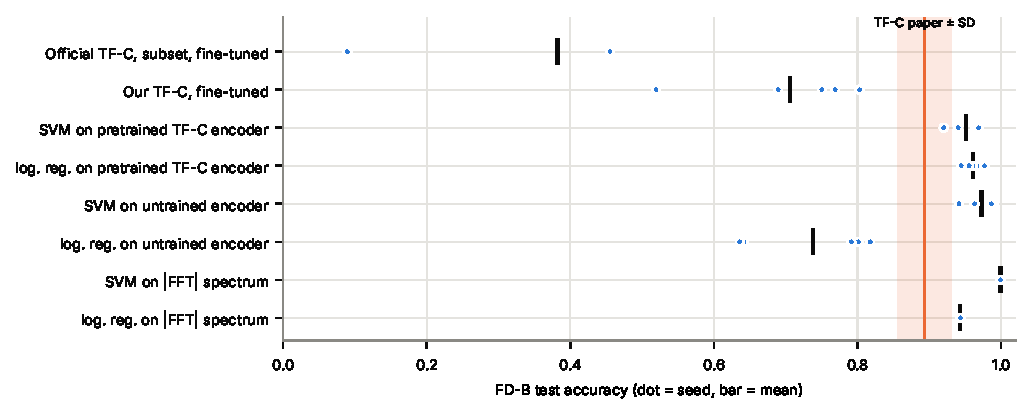
\includegraphics[width=\linewidth]{fdb_overview}
\caption{FD-B test accuracy for every TF-C model and probe: dots are seeds, bars
means. Shaded: published TF-C accuracy $\pm$ SD.}
\label{fig:fdb}
\end{figure}

\begin{figure}[htbp]
\centering
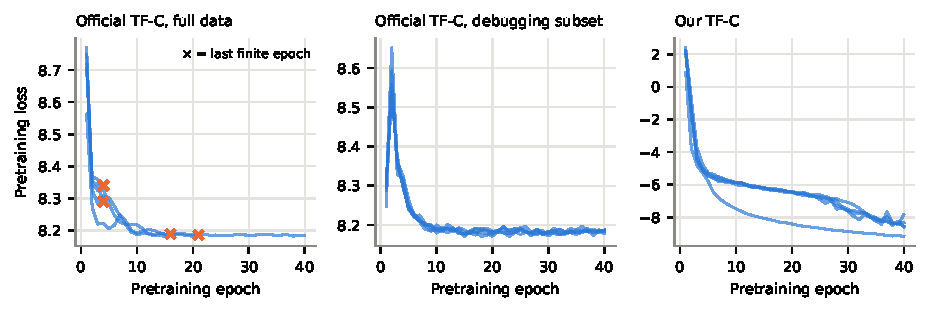
\includegraphics[width=\linewidth]{tfc_pretrain_loss}
\caption{TF-C pretraining loss per epoch, one line per seed. Left: official code, full data
(third attempt); $\times$ marks the last finite epoch. Middle: official code, debugging
subset. Right: our TF-C; its loss is defined differently (D41 item 4), so the
scales are not comparable.}
\label{fig:tfc-loss}
\end{figure}

% =============================================================================
\section{Herning test rig}

The Herning run \run{scope_20260901_112732} is a validation run of an unfinished rig (D7,
D22): one bearing, one lubricant, rpm swept up and down at 13 temperature targets. The
regression target is $\kappa$, computed from rpm and temperature as in the MSSP code (D55).
Figure~\ref{fig:herning-op} shows the operating points.

\begin{figure}[htbp]
\centering
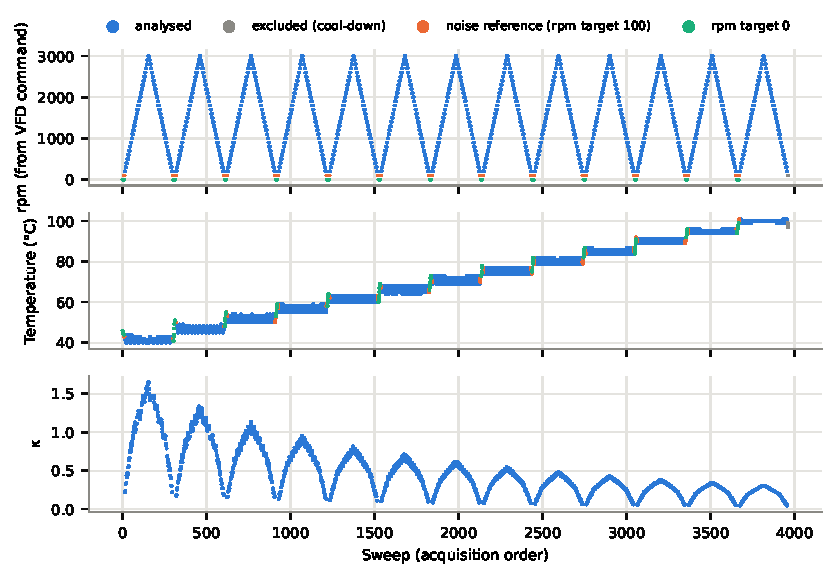
\includegraphics[width=\linewidth]{herning_operating_points}
\caption{Herning run: rpm (from the frequency-converter command), temperature and $\kappa$
for every sweep, in acquisition order, coloured by role in the band check (\sref{band-check}; D52, D55).}
\label{fig:herning-op}
\end{figure}

\entry{band-check}{Herning band check: where AE and US carry information}{2026-10-09}
  {D51, D52, D55; led to D60, D61, D62, Q3}{\run{20261009_085307_band_check_herning}}

\question
Before band-limiting and downsampling the rig signals (D51): in which frequency bands do
AE and US carry signal from the rotating bearing, and does that signal depend on the
operating point (D52)?

\test
\texttt{eda/herning/check\_bands.py} (then in \texttt{scripts/}; moved by D68) on the source file. Per sweep and sensor: Welch power
spectrum (Hann window, 65,536 samples, 50\,\% overlap; 38-Hz resolution at 2.5 MHz),
integrated over a low band (0--891 Hz) and base-10 third-octave bands from 1 kHz to
Nyquist. Sweeps: \BandSweeps{} in total; \BandAnalysed{} analysed (rotating, D55
exclusions applied), \BandNoise{} noise reference (rpm target 100: bearing not rotating),
\BandZero{} at rpm target 0, \BandExcluded{} excluded (cool-down). Per band: ratio of the
median power of analysed sweeps to the noise reference (dB), and Spearman correlation of
band power with rpm, temperature and $\kappa$ ($\kappa$ from \BandKappaMin{} to
\BandKappaMax). Extra control against slow drift over the 13-hour run: the correlation with
rpm computed within each temperature block (median over blocks). Run in four chunks of
sweeps (3-minute limit per call), merged into one result (\texttt{NOTE.txt}). An earlier
folder (\run{20261009_085150_band_check_herning}) contains only the config.

\result
Figure~\ref{fig:bands}; all bands in Table~\ref{tab:bands} (Appendix~\ref{app:bands}).
\begin{itemize}
  \item AE: power above the reference from about 12.6 kHz to about 400 kHz, with peaks of
        \BandAePeakLow{} and \BandAePeakHigh. In the bands from 12.6 to 398 kHz the
        within-block correlation with rpm is \BandAeCoreRpm. From 631 kHz up there is no
        excess power (at most \BandAeTopDb~dB) and band power \emph{falls} with rpm within
        blocks ($\rho$ from \BandAeTopRpm).
  \item US: \BandUsLowDb~dB above the reference up to 6.3 kHz. Between about 40 and 200 kHz
        the excess is only \BandUsMidDb~dB, but band power still rises with rpm within
        blocks ($\rho$ \BandUsMidRpm) and correlates with $\kappa$ ($\rho$ \BandUsMidKappa).
\end{itemize}

\finding
AE shows rpm-dependent power above the reference roughly between 12 and 560 kHz (the
origin of the part below 50 kHz is unknown, D60); above about 560 kHz it shows no excess
power, and the user regards it as noise (D61, D62). US carries most of its power below about 8 kHz, but rpm-dependent content continues
up to about 200 kHz. Correlation within temperature blocks rules out slow drift, but not
electrical interference that also scales with speed (Q3).

\consequence
Feature bands: AE 50--560 kHz (nothing below the 50-kHz coupler high-pass; D60, D61), US
0.71--178 kHz (D60). Downsampling: AE by 2 (1.25 MHz), US by 5 (500 kHz) (D62). Whether US
above about 40 kHz is bearing signal or interference is open (Q3).

\begin{figure}[htbp]
\centering
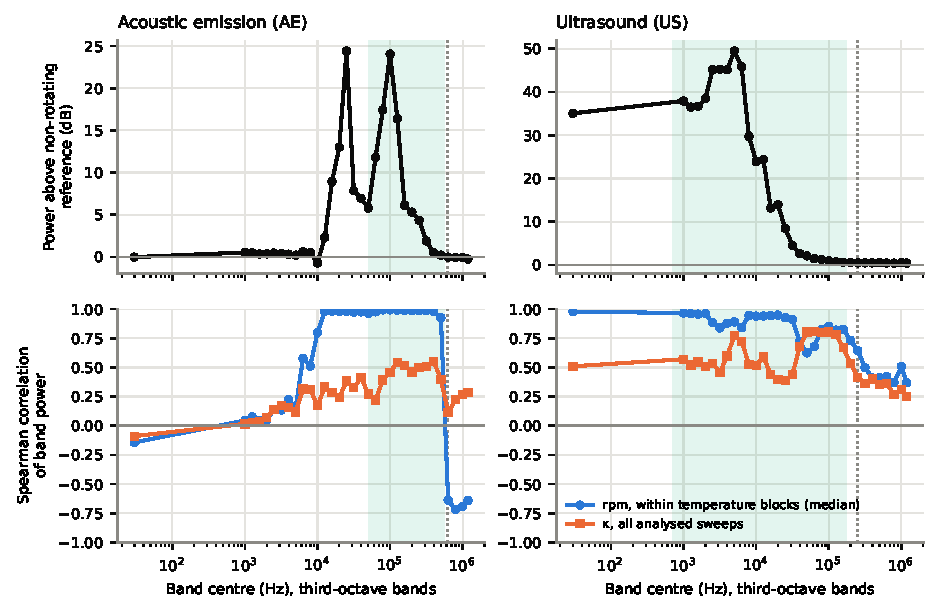
\includegraphics[width=\linewidth]{herning_band_check}
\caption{Herning band check. Top: median band power of rotating sweeps relative to
the non-rotating reference. Bottom: Spearman correlation of band power with rpm (median
within temperature blocks) and with $\kappa$ (all analysed sweeps). Shaded: feature bands
(D60, D61). Dotted: Nyquist frequency after downsampling (D62). The leftmost point is the
0--891-Hz band.}
\label{fig:bands}
\end{figure}

% =============================================================================
\section{Open points}

From this document:
\begin{itemize}
  \item Data layer (\sref{data-conversion}): test outcomes are not stored as files.
  \item FordA (\sref{forda-baselines}): TS-JEPA and PatchTST not yet in the comparison; the
        untrained-encoder control (D75 f) not run.
  \item Official TF-C, full data (\sref{tfc-full}): why seed 4 has no fine-tuning output.
  \item Our TF-C (\sref{tfc-ours}): whether it counts as a reproduction, and whether the
        reproduction criterion needs a condition on the spread.
  \item FD-B (\sref{fdb-spectrum}): what follows for the TF-C study (D35) from the FD-B
        diagnostics.
\end{itemize}
For supervision (\texttt{QUESTIONS.md}): Q1 Herning split (temperature hold-out details);
Q2 comparing whole-sweep features with window-based SSL representations; Q3 US above
40 kHz and AE above 560 kHz --- bearing signal or electrical interference.

% =============================================================================
\appendix

\section{Run index}\label{app:runs}

% Generated by scripts/make_report.py - do not edit by hand.
\begin{footnotesize}
\begin{longtable}{>{\raggedright\arraybackslash}p{0.28\linewidth}>{\raggedright\arraybackslash}p{0.22\linewidth}>{\raggedright\arraybackslash}p{0.22\linewidth}ll}
\caption{Run index: every folder in \texttt{runs/} (D98). Commit with $^{*}$: the working tree had uncommitted changes when the run started, so the commit alone does not reproduce the code.}\label{tab:runs}\\
\toprule
Run folder (\texttt{runs/}) & What & Status & Commit & Device \\
\midrule
\endfirsthead
\toprule
Run folder (\texttt{runs/}) & What & Status & Commit & Device \\
\midrule
\endhead
\texttt{20261007\_\allowbreak{}214220\_\allowbreak{}ts2vec\_\allowbreak{}forda\_\allowbreak{}cpu\_\allowbreak{}check} & TS2Vec on FordA, CPU check in the cloud workspace & Superseded by 20261008\_\allowbreak{}084722\_\allowbreak{}ts2vec\_\allowbreak{}forda & none$^{*}$ & cpu \\
\texttt{20261008\_\allowbreak{}084722\_\allowbreak{}ts2vec\_\allowbreak{}forda} & TS2Vec on FordA (reproduction) & Superseded by 20261020\_\allowbreak{}144711\_\allowbreak{}ts2vec\_\allowbreak{}forda (rerun with timing) & adf16c6 & cuda \\
\texttt{20261008\_\allowbreak{}092321\_\allowbreak{}tloss\_\allowbreak{}forda} & T-Loss on FordA (reproduction) & Superseded by 20261020\_\allowbreak{}144932\_\allowbreak{}tloss\_\allowbreak{}forda (rerun with timing) & 5320251$^{*}$ & cuda \\
\texttt{20261008\_\allowbreak{}134951\_\allowbreak{}tfc\_\allowbreak{}official\_\allowbreak{}fd} & Official TF-C, full FD-A data, attempt 1 & In \S\ref{tfc-full} & 87e9222$^{*}$ & cuda \\
\texttt{20261008\_\allowbreak{}142751\_\allowbreak{}tfc\_\allowbreak{}fd} & Our TF-C, FD-A to FD-B & In \S\ref{tfc-ours} & 87e9222$^{*}$ & cuda \\
\texttt{20261008\_\allowbreak{}143021\_\allowbreak{}tfc\_\allowbreak{}official\_\allowbreak{}fd} & Official TF-C, full FD-A data, attempt 2 & In \S\ref{tfc-full} & 87e9222$^{*}$ & cuda \\
\texttt{20261008\_\allowbreak{}151014\_\allowbreak{}probe\_\allowbreak{}tfc\_\allowbreak{}fd} & Frozen probes on our TF-C encoders & In \S\ref{tfc-probe} & 87e9222$^{*}$ & cuda \\
\texttt{20261008\_\allowbreak{}155516\_\allowbreak{}tfc\_\allowbreak{}official\_\allowbreak{}fd} & Official TF-C, full FD-A data, attempt 3 & In \S\ref{tfc-full} & c11957a$^{*}$ & cuda \\
\texttt{20261008\_\allowbreak{}162447\_\allowbreak{}probe\_\allowbreak{}spectrum\_\allowbreak{}fd} & Probes on the $|$FFT$|$ spectra of FD-B & In \S\ref{fdb-spectrum} & none & -- \\
\texttt{20261008\_\allowbreak{}171159\_\allowbreak{}tfc\_\allowbreak{}official\_\allowbreak{}fd\_\allowbreak{}subset} & Official TF-C, debugging subset & In \S\ref{tfc-subset} & c11957a$^{*}$ & cuda \\
\texttt{20261009\_\allowbreak{}085150\_\allowbreak{}band\_\allowbreak{}check\_\allowbreak{}herning} & Herning band check, stopped before writing results & Empty & c11957a$^{*}$ & -- \\
\texttt{20261009\_\allowbreak{}085307\_\allowbreak{}band\_\allowbreak{}check\_\allowbreak{}herning} & Herning band check & In \S\ref{band-check} & c11957a$^{*}$ & -- \\
\texttt{20261012\_\allowbreak{}205347\_\allowbreak{}spectra\_\allowbreak{}herning} & Herning spectra & Examination (QUESTIONS.md, Q3) & 5dba814$^{*}$ & -- \\
\texttt{20261012\_\allowbreak{}210217\_\allowbreak{}vfd\_\allowbreak{}lines\_\allowbreak{}herning} & Frequency-converter lines in the Herning spectra & Examination (QUESTIONS.md, Q3) & 5dba814$^{*}$ & -- \\
\texttt{20261014\_\allowbreak{}herning\_\allowbreak{}examination} & Herning dataset examination & Examination (eda/herning) & -- & -- \\
\texttt{20261016\_\allowbreak{}114600\_\allowbreak{}tsjepa\_\allowbreak{}forda} & TS-JEPA on FordA & Not written up yet & 5bde87a$^{*}$ & cuda \\
\texttt{20261016\_\allowbreak{}114616\_\allowbreak{}tsjepa\_\allowbreak{}forda\_\allowbreak{}fixed} & TS-JEPA (masking fixed) on FordA & Not written up yet & 5bde87a$^{*}$ & cuda \\
\texttt{20261017\_\allowbreak{}115419\_\allowbreak{}collapse\_\allowbreak{}forda} & Collapse check on FordA & Not written up yet & 7a69724$^{*}$ & cuda \\
\texttt{20261019\_\allowbreak{}130910\_\allowbreak{}patchtst\_\allowbreak{}forda} & PatchTST on FordA & Not written up yet & 7a69724$^{*}$ & cuda \\
\texttt{20261019\_\allowbreak{}154248\_\allowbreak{}patchtst\_\allowbreak{}forda\_\allowbreak{}mean} & PatchTST re-encoded with mean pooling (D86, D87) & Not written up yet & none$^{*}$ & cpu \\
\texttt{20261019\_\allowbreak{}154305\_\allowbreak{}patchtst\_\allowbreak{}forda\_\allowbreak{}flatten} & PatchTST re-encoded with flatten pooling (D86) & Not written up yet & none$^{*}$ & cpu \\
\texttt{20261020\_\allowbreak{}135846\_\allowbreak{}ablation\_\allowbreak{}forda\_\allowbreak{}A} & TF-C ablation on FordA, step A & Not written up yet & beee5e8$^{*}$ & cuda \\
\texttt{20261020\_\allowbreak{}140639\_\allowbreak{}ablation\_\allowbreak{}forda\_\allowbreak{}B} & TF-C ablation on FordA, step B & Not written up yet & beee5e8$^{*}$ & cuda \\
\texttt{20261020\_\allowbreak{}141430\_\allowbreak{}ablation\_\allowbreak{}forda\_\allowbreak{}C} & TF-C ablation on FordA, step C & Not written up yet & beee5e8$^{*}$ & cuda \\
\texttt{20261020\_\allowbreak{}143928\_\allowbreak{}raw\_\allowbreak{}forda} & Baseline: raw samples (and floor) on FordA & In \S\ref{forda-baselines} & beee5e8$^{*}$ & cpu \\
\texttt{20261020\_\allowbreak{}144122\_\allowbreak{}fft\_\allowbreak{}forda} & Baseline: $|$FFT$|$ on FordA & In \S\ref{forda-baselines} & beee5e8$^{*}$ & cpu \\
\texttt{20261020\_\allowbreak{}144235\_\allowbreak{}catch22\_\allowbreak{}forda} & Baseline: catch24 on FordA & In \S\ref{forda-baselines} & beee5e8$^{*}$ & cpu \\
\texttt{20261020\_\allowbreak{}144711\_\allowbreak{}ts2vec\_\allowbreak{}forda} & TS2Vec on FordA, with timing & In \S\ref{forda-repro}, \S\ref{forda-baselines} & beee5e8$^{*}$ & cuda \\
\texttt{20261020\_\allowbreak{}144932\_\allowbreak{}tloss\_\allowbreak{}forda} & T-Loss on FordA, with timing & In \S\ref{forda-repro}, \S\ref{forda-baselines} & beee5e8$^{*}$ & cuda \\
\texttt{20261020\_\allowbreak{}152809\_\allowbreak{}minirocket\_\allowbreak{}forda} & Baseline: MiniRocket on FordA & In \S\ref{forda-repro}, \S\ref{forda-baselines} & beee5e8$^{*}$ & cpu \\
\texttt{20261021\_\allowbreak{}104231\_\allowbreak{}ablation\_\allowbreak{}forda\_\allowbreak{}D} & -- & Not indexed & 40618b6 & cuda \\
\bottomrule
\end{longtable}
\end{footnotesize}


\section{Herning band check: all bands}\label{app:bands}

% Generated by scripts/make_report.py - do not edit by hand.
\begin{small}
\begin{longtable}{llrrrrr}
\caption{Herning band check, all bands. Ratio: median band power of analysed sweeps over that of the non-rotating reference. $\rho$: Spearman correlation of band power with rpm (all analysed sweeps, and median within temperature blocks), temperature and $\kappa$.}\label{tab:bands}\\
\toprule
Sensor & Band & Ratio (dB) & $\rho$ rpm & $\rho$ rpm in block & $\rho$ temp. & $\rho$ $\kappa$ \\
\midrule
\endfirsthead
\toprule
Sensor & Band & Ratio (dB) & $\rho$ rpm & $\rho$ rpm in block & $\rho$ temp. & $\rho$ $\kappa$ \\
\midrule
\endhead
AE & 0-891.25 Hz & $-0.0$ & $-0.08$ & $-0.14$ & $0.13$ & $-0.09$ \\
AE & 1 kHz & $0.5$ & $0.03$ & $0.04$ & $0.10$ & $0.02$ \\
AE & 1.259 kHz & $0.5$ & $0.06$ & $0.08$ & $0.12$ & $0.03$ \\
AE & 1.585 kHz & $0.3$ & $0.04$ & $0.05$ & $0.08$ & $0.04$ \\
AE & 1.995 kHz & $0.4$ & $0.07$ & $0.05$ & $0.07$ & $0.07$ \\
AE & 2.512 kHz & $0.5$ & $0.16$ & $0.14$ & $0.04$ & $0.14$ \\
AE & 3.162 kHz & $0.4$ & $0.16$ & $0.13$ & $-0.01$ & $0.17$ \\
AE & 3.981 kHz & $0.3$ & $0.20$ & $0.22$ & $0.04$ & $0.15$ \\
AE & 5.012 kHz & $0.2$ & $0.08$ & $0.16$ & $0.00$ & $0.12$ \\
AE & 6.31 kHz & $0.6$ & $0.55$ & $0.58$ & $0.09$ & $0.31$ \\
AE & 7.943 kHz & $0.5$ & $0.48$ & $0.51$ & $0.05$ & $0.31$ \\
AE & 10 kHz & $-0.7$ & $0.70$ & $0.80$ & $0.30$ & $0.17$ \\
AE & 12.59 kHz & $2.3$ & $0.90$ & $0.98$ & $0.29$ & $0.33$ \\
AE & 15.85 kHz & $8.9$ & $0.88$ & $0.98$ & $0.35$ & $0.29$ \\
AE & 19.95 kHz & $13.0$ & $0.86$ & $0.98$ & $0.40$ & $0.24$ \\
AE & 25.12 kHz & $24.4$ & $0.90$ & $0.98$ & $0.24$ & $0.38$ \\
AE & 31.62 kHz & $7.8$ & $0.87$ & $0.97$ & $0.29$ & $0.32$ \\
AE & 39.81 kHz & $6.9$ & $0.91$ & $0.98$ & $0.20$ & $0.41$ \\
AE & 50.12 kHz & $5.8$ & $0.86$ & $0.96$ & $0.35$ & $0.27$ \\
AE & 63.1 kHz & $11.8$ & $0.85$ & $0.98$ & $0.42$ & $0.22$ \\
AE & 79.43 kHz & $17.4$ & $0.95$ & $0.99$ & $0.25$ & $0.39$ \\
AE & 100 kHz & $24.0$ & $0.96$ & $0.99$ & $0.17$ & $0.46$ \\
AE & 125.9 kHz & $16.4$ & $0.98$ & $0.99$ & $0.07$ & $0.54$ \\
AE & 158.5 kHz & $6.1$ & $0.97$ & $0.99$ & $0.11$ & $0.51$ \\
AE & 199.5 kHz & $5.3$ & $0.96$ & $0.99$ & $0.17$ & $0.46$ \\
AE & 251.2 kHz & $4.3$ & $0.97$ & $0.99$ & $0.12$ & $0.50$ \\
AE & 316.2 kHz & $1.9$ & $0.96$ & $0.99$ & $0.11$ & $0.51$ \\
AE & 398.1 kHz & $0.5$ & $0.97$ & $0.98$ & $0.05$ & $0.55$ \\
AE & 501.2 kHz & $0.2$ & $0.83$ & $0.93$ & $0.16$ & $0.40$ \\
AE & 631 kHz & $-0.0$ & $-0.43$ & $-0.64$ & $-0.34$ & $0.11$ \\
AE & 794.3 kHz & $-0.1$ & $-0.33$ & $-0.72$ & $-0.46$ & $0.22$ \\
AE & 1000 kHz & $-0.1$ & $-0.27$ & $-0.69$ & $-0.49$ & $0.27$ \\
AE & 1259 kHz & $-0.2$ & $-0.25$ & $-0.64$ & $-0.50$ & $0.28$ \\
US & 0-891.25 Hz & $35.0$ & $0.96$ & $0.98$ & $0.09$ & $0.51$ \\
US & 1 kHz & $37.9$ & $0.96$ & $0.97$ & $0.02$ & $0.57$ \\
US & 1.259 kHz & $36.5$ & $0.93$ & $0.96$ & $0.07$ & $0.52$ \\
US & 1.585 kHz & $36.7$ & $0.94$ & $0.96$ & $0.04$ & $0.55$ \\
US & 1.995 kHz & $38.4$ & $0.95$ & $0.96$ & $0.09$ & $0.51$ \\
US & 2.512 kHz & $45.1$ & $0.85$ & $0.88$ & $-0.00$ & $0.53$ \\
US & 3.162 kHz & $45.3$ & $0.82$ & $0.84$ & $0.07$ & $0.46$ \\
US & 3.981 kHz & $45.1$ & $0.84$ & $0.88$ & $-0.09$ & $0.60$ \\
US & 5.012 kHz & $49.5$ & $0.81$ & $0.89$ & $-0.31$ & $0.77$ \\
US & 6.31 kHz & $45.8$ & $0.78$ & $0.84$ & $-0.26$ & $0.72$ \\
US & 7.943 kHz & $29.7$ & $0.91$ & $0.94$ & $0.06$ & $0.53$ \\
US & 10 kHz & $23.9$ & $0.91$ & $0.94$ & $0.06$ & $0.52$ \\
US & 12.59 kHz & $24.4$ & $0.90$ & $0.94$ & $-0.03$ & $0.59$ \\
US & 15.85 kHz & $13.1$ & $0.88$ & $0.94$ & $0.15$ & $0.44$ \\
US & 19.95 kHz & $13.9$ & $0.88$ & $0.95$ & $0.21$ & $0.40$ \\
US & 25.12 kHz & $8.4$ & $0.85$ & $0.93$ & $0.21$ & $0.39$ \\
US & 31.62 kHz & $4.5$ & $0.85$ & $0.91$ & $0.14$ & $0.44$ \\
US & 39.81 kHz & $2.6$ & $0.64$ & $0.72$ & $-0.25$ & $0.68$ \\
US & 50.12 kHz & $2.1$ & $0.60$ & $0.62$ & $-0.42$ & $0.80$ \\
US & 63.1 kHz & $1.4$ & $0.63$ & $0.68$ & $-0.42$ & $0.81$ \\
US & 79.43 kHz & $1.3$ & $0.76$ & $0.82$ & $-0.35$ & $0.80$ \\
US & 100 kHz & $0.9$ & $0.78$ & $0.85$ & $-0.35$ & $0.80$ \\
US & 125.9 kHz & $0.7$ & $0.74$ & $0.82$ & $-0.36$ & $0.78$ \\
US & 158.5 kHz & $0.6$ & $0.79$ & $0.83$ & $-0.21$ & $0.67$ \\
US & 199.5 kHz & $0.6$ & $0.71$ & $0.73$ & $-0.11$ & $0.53$ \\
US & 251.2 kHz & $0.5$ & $0.64$ & $0.64$ & $-0.01$ & $0.42$ \\
US & 316.2 kHz & $0.5$ & $0.53$ & $0.50$ & $-0.03$ & $0.36$ \\
US & 398.1 kHz & $0.5$ & $0.40$ & $0.41$ & $-0.15$ & $0.40$ \\
US & 501.2 kHz & $0.5$ & $0.37$ & $0.41$ & $-0.11$ & $0.35$ \\
US & 631 kHz & $0.4$ & $0.40$ & $0.42$ & $-0.10$ & $0.36$ \\
US & 794.3 kHz & $0.4$ & $0.37$ & $0.37$ & $-0.01$ & $0.27$ \\
US & 1000 kHz & $0.5$ & $0.51$ & $0.51$ & $0.04$ & $0.31$ \\
US & 1259 kHz & $0.4$ & $0.38$ & $0.37$ & $0.01$ & $0.25$ \\
\bottomrule
\end{longtable}
\end{small}


\end{document}
